% Strip plot of clinician survey responses — n=5 raters, 4 real sub-groups.
% Rightmost column: six decoy groups pooled as a box plot (n=30 per dimension).
% Real groups: individual dots + range bar + mean bar.
% Decoy pool: IQR box (Q1--Q3) + whiskers (min/max) + mean bar.
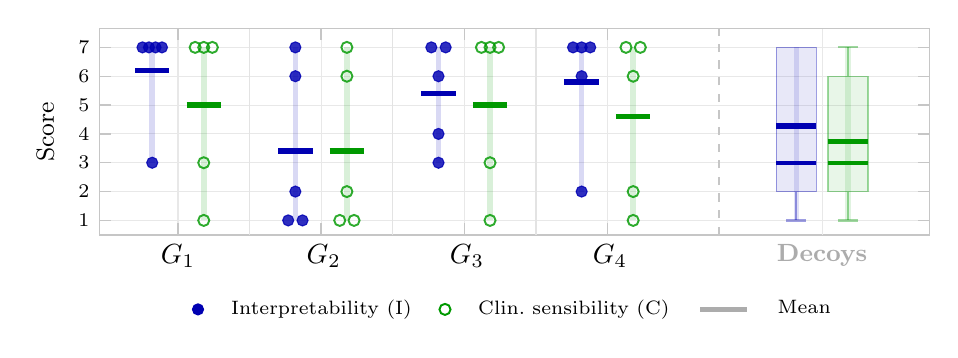
\begin{tikzpicture}
\begin{axis}[
  width=\columnwidth,
  height=4.2cm,
  xmin=0.45, xmax=6.25,
  ymin=0.5,  ymax=7.65,
  ytick={1,...,7},
  xtick={1,2,3,4},
  xticklabels={$G_1$,\,$G_2$,\,$G_3$,\,$G_4$},
  extra x ticks={5.5},
  extra x tick labels={Decoys},
  extra x tick style={
    tick style={draw=none},
    xticklabel style={font=\small\bfseries, text=gray!65},
  },
  ylabel={Score},
  ylabel style={font=\small, yshift=2pt},
  yticklabel style={font=\scriptsize},
  xticklabel style={font=\small, font=\bfseries},
  grid=major,
  grid style={draw=gray!18, line width=0.4pt},
  axis line style={draw=gray!45, line width=0.5pt},
  tick style={draw=gray!45, line width=0.5pt},
  clip=false,
  legend style={
    at={(0.5,-0.26)},
    anchor=north,
    legend columns=3,
    font=\scriptsize,
    draw=none,
    fill=none,
    column sep=8pt,
  },
]

%% ---- Group separators (real groups) --------------------------------
\foreach \sep in {1.5, 2.5, 3.5} {
  \addplot[color=gray!22, line width=0.5pt, forget plot]
    coordinates {(\sep,0.5) (\sep,7.65)};
}

%% ---- Separator: real groups vs. decoy pool -------------------------
\addplot[color=gray!45, line width=0.7pt, dashed, forget plot]
  coordinates {(4.78,0.5) (4.78,7.65)};

%% ---- Range bars (min--max, real groups) ----------------------------
% Interpretability
\addplot[color=blue!70!black, line width=2pt, opacity=0.15, forget plot]
  coordinates {(0.82,3)(0.82,7)};
\addplot[color=blue!70!black, line width=2pt, opacity=0.15, forget plot]
  coordinates {(1.82,1)(1.82,7)};
\addplot[color=blue!70!black, line width=2pt, opacity=0.15, forget plot]
  coordinates {(2.82,3)(2.82,7)};
\addplot[color=blue!70!black, line width=2pt, opacity=0.15, forget plot]
  coordinates {(3.82,2)(3.82,7)};
% Clinical sensibility
\addplot[color=green!60!black, line width=2pt, opacity=0.15, forget plot]
  coordinates {(1.18,1)(1.18,7)};
\addplot[color=green!60!black, line width=2pt, opacity=0.15, forget plot]
  coordinates {(2.18,1)(2.18,7)};
\addplot[color=green!60!black, line width=2pt, opacity=0.15, forget plot]
  coordinates {(3.18,1)(3.18,7)};
\addplot[color=green!60!black, line width=2pt, opacity=0.15, forget plot]
  coordinates {(4.18,1)(4.18,7)};

%% ---- Interpretability dots (filled circles) -----------------------
%  Jitter applied to identical values within the same sub-column.
%  Data: G1=[3,7,7,7,7]  G2=[2,1,7,1,6]  G3=[3,7,7,6,4]  G4=[2,7,7,7,6]
\addplot[only marks, mark=*, mark size=2.0pt,
         color=blue!70!black, opacity=0.82, forget plot] coordinates {
  % G1
  (0.820,3)
  (0.752,7)(0.797,7)(0.843,7)(0.888,7)
  % G2
  (1.770,1)(1.870,1)
  (1.820,2)(1.820,6)(1.820,7)
  % G3
  (2.820,3)(2.820,4)(2.820,6)
  (2.770,7)(2.870,7)
  % G4
  (3.820,2)(3.820,6)
  (3.760,7)(3.820,7)(3.880,7)
};

%% ---- Clinical Sensibility dots (open circles) ---------------------
%  Data: G1=[3,7,7,1,7]  G2=[2,1,7,1,6]  G3=[3,7,7,1,7]  G4=[1,7,7,2,6]
\addplot[only marks, mark=o, mark size=2.0pt, line width=0.7pt,
         color=green!60!black, opacity=0.82, forget plot] coordinates {
  % G1
  (1.180,1)(1.180,3)
  (1.120,7)(1.180,7)(1.240,7)
  % G2
  (2.130,1)(2.230,1)
  (2.180,2)(2.180,6)(2.180,7)
  % G3
  (3.180,1)(3.180,3)
  (3.120,7)(3.180,7)(3.240,7)
  % G4
  (4.180,1)(4.180,2)(4.180,6)
  (4.130,7)(4.230,7)
};

%% ---- Mean bars (real groups) ---------------------------------------
% G1: interp=6.2, clin=5.0
\addplot[color=blue!70!black,  line width=2pt, mark=none, forget plot]
  coordinates {(0.70,6.2)(0.94,6.2)};
\addplot[color=green!60!black, line width=2pt, mark=none, forget plot]
  coordinates {(1.06,5.0)(1.30,5.0)};
% G2: interp=3.4, clin=3.4
\addplot[color=blue!70!black,  line width=2pt, mark=none, forget plot]
  coordinates {(1.70,3.4)(1.94,3.4)};
\addplot[color=green!60!black, line width=2pt, mark=none, forget plot]
  coordinates {(2.06,3.4)(2.30,3.4)};
% G3: interp=5.4, clin=5.0
\addplot[color=blue!70!black,  line width=2pt, mark=none, forget plot]
  coordinates {(2.70,5.4)(2.94,5.4)};
\addplot[color=green!60!black, line width=2pt, mark=none, forget plot]
  coordinates {(3.06,5.0)(3.30,5.0)};
% G4: interp=5.8, clin=4.6
\addplot[color=blue!70!black,  line width=2pt, mark=none, forget plot]
  coordinates {(3.70,5.8)(3.94,5.8)};
\addplot[color=green!60!black, line width=2pt, mark=none, forget plot]
  coordinates {(4.06,4.6)(4.30,4.6)};

%% ---- Decoy pool: range lines (both dims span 1--7) ----------------
\addplot[color=blue!70!black,  line width=2pt, opacity=0.12, forget plot]
  coordinates {(5.32,1)(5.32,7)};
\addplot[color=green!60!black, line width=2pt, opacity=0.12, forget plot]
  coordinates {(5.68,1)(5.68,7)};

%% ---- Decoy pool: IQR boxes ----------------------------------------
% Interpretability (Q1=2, Q3=7)
\fill[blue!70!black, opacity=0.09]
  (axis cs:5.18,2) rectangle (axis cs:5.46,7);
\draw[blue!70!black, line width=0.5pt, opacity=0.38]
  (axis cs:5.18,2) rectangle (axis cs:5.46,7);
% Clinical Sensibility (Q1=2, Q3=6)
\fill[green!60!black, opacity=0.09]
  (axis cs:5.54,2) rectangle (axis cs:5.82,6);
\draw[green!60!black, line width=0.5pt, opacity=0.38]
  (axis cs:5.54,2) rectangle (axis cs:5.82,6);

%% ---- Decoy pool: whiskers -----------------------------------------
% Interpretability: lower whisker only (Q1=2 to min=1; Q3=max=7, no upper)
\draw[blue!70!black, line width=0.8pt, opacity=0.38]
  (axis cs:5.32,2) -- (axis cs:5.32,1);
\draw[blue!70!black, line width=0.8pt, opacity=0.38]
  (axis cs:5.25,1) -- (axis cs:5.39,1);
% Clinical Sensibility: lower (Q1=2 to min=1) and upper (Q3=6 to max=7)
\draw[green!60!black, line width=0.8pt, opacity=0.38]
  (axis cs:5.68,2) -- (axis cs:5.68,1);
\draw[green!60!black, line width=0.8pt, opacity=0.38]
  (axis cs:5.61,1) -- (axis cs:5.75,1);
\draw[green!60!black, line width=0.8pt, opacity=0.38]
  (axis cs:5.68,6) -- (axis cs:5.68,7);
\draw[green!60!black, line width=0.8pt, opacity=0.38]
  (axis cs:5.61,7) -- (axis cs:5.75,7);

%% ---- Decoy pool: median lines (median=3 for both) -----------------
\draw[blue!70!black,  line width=1.6pt]
  (axis cs:5.18,3) -- (axis cs:5.46,3);
\draw[green!60!black, line width=1.6pt]
  (axis cs:5.54,3) -- (axis cs:5.82,3);

%% ---- Decoy pool: mean bars (same style as real groups) ------------
% Interpretability mean = 4.27
\addplot[color=blue!70!black,  line width=2pt, mark=none, forget plot]
  coordinates {(5.18,4.27)(5.46,4.27)};
% Clinical Sensibility mean = 3.73
\addplot[color=green!60!black, line width=2pt, mark=none, forget plot]
  coordinates {(5.54,3.73)(5.82,3.73)};


%% ---- Legend -------------------------------------------------------
\addlegendimage{only marks, mark=*, color=blue!70!black, mark size=2.0pt}
\addlegendentry{Interpretability~(I)}
\addlegendimage{only marks, mark=o, color=green!60!black,
                mark size=2.0pt, line width=0.7pt}
\addlegendentry{Clin.\ sensibility~(C)}
\addlegendimage{color=gray!65, line width=2pt}
\addlegendentry{Mean}

\end{axis}
\end{tikzpicture}
